\subsection{Analytics Parameter Study Experiments}

One of the important aspects of analytics as a service is the ability to integrate long running analytics tasks either 
on the current computer, remote computers or batch queuing systems from HPC tasks. Theses tasks can be 
executed directly on the host system but can simplify access for the user by placing them behind REST 
services. This is is a common compute pattern as part of parameter studies that explore a variety of 
parameters producing analytics results that can then be explored either in collaboration or competition. 

To achieve this goal a primary execution pattern for this case is outlined as follows:


\begin{enumerate}
    \item Provisioning one or multiple compute Node on which the parameter experiment is conducted.
    \item Create hyperparameters for the analytics calculation suitable for the compute resources.
    \item Prepare the compute resources with the needed data and programs to conduct the analytics 
          functions. This can be done by copying the source to the nodes, or using a GitHub repository to 
          obtain the source.
    \item Configuring the system's software to prepare for a benchmark run by installing or compiling the code 
          in a way that is best suited for the resource).
    % \item Start GPU monitoring to begin capturing GPU metadata
    \item Executing the analytics function and capturing the results
\end{enumerate}

This logic is captured as part of the analytics paratmeter experiment  management and is implemented using the Cloudmesh-Sbatch utility specifically targeting execution pattern \cite{repo-cloudmesh-sbatch}.
This utility provides the ability to specify configurable parameters that perform one-to-one substitutions and a special \textit{experiments} parameter set, which creates a permutation for all parameter values as distinct experiments.

This allows the user to provide a single script with a configuration file containing multiple hyperparameter values and have them expand into hundreds of configurations without having to prepare each configuration manually.
A typical workflow of development is illustated in Figure \ref{fig:sbatch} and Figure \ref{fig:sbatch-submit}.

\begin{figure*}[htb]
    \centering
    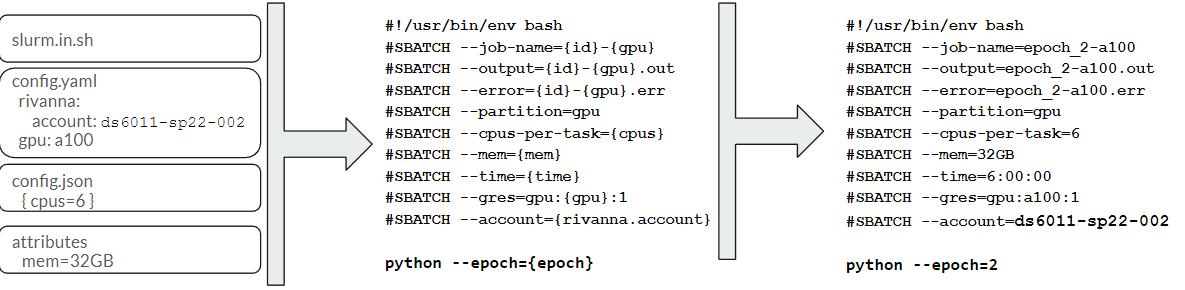
\includegraphics[width=0.8\textwidth]{images/sbatch-template.png}
    \caption{SBatch Generation Workflow}\label{fig:sbatch}

    \centering
    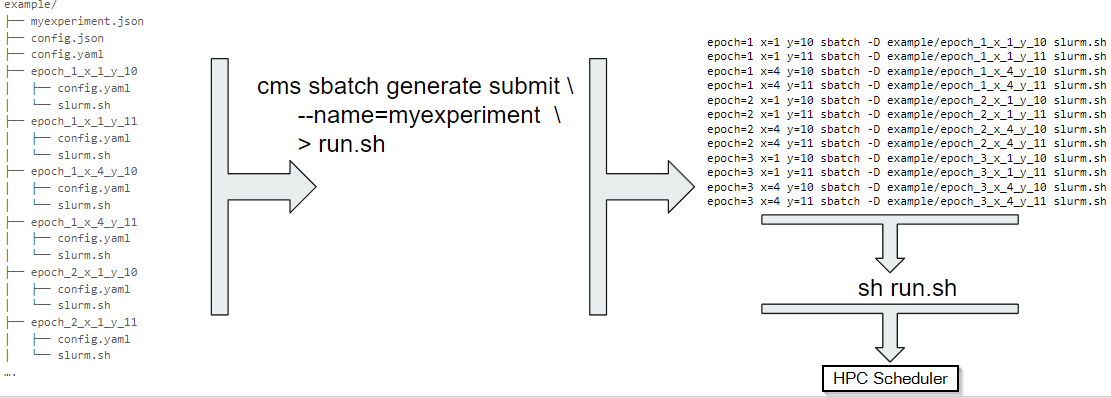
\includegraphics[width=0.8\textwidth]{images/sbatch-submit.png}
    \caption{SBatch Submission Workflow}\label{fig:sbatch-submit}

    \centering
    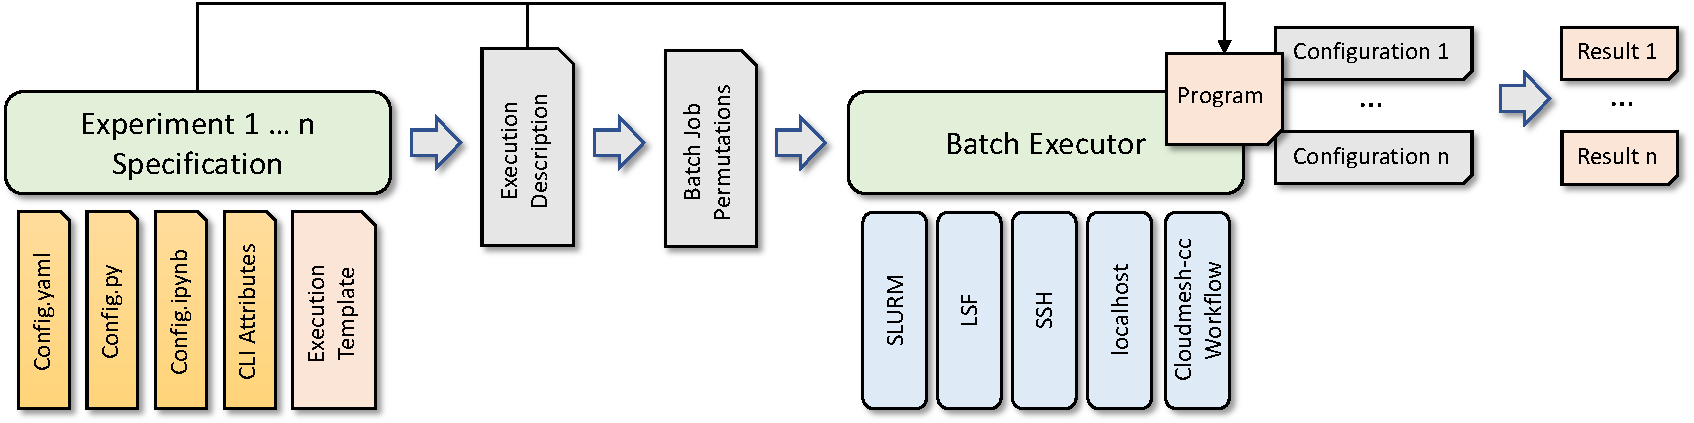
\includegraphics[width=0.8\textwidth]{images/sbatch.pdf}
    \caption{SBatch Sumission Workflow}\label{fig:sbatch-2}
\end{figure*}


